\documentclass{standalone}
\usepackage{graphicx}
\usepackage{subcaption}
\usepackage{tikz}

\begin{document}

\begin{tikzpicture}
    % First figure
    \node[draw, rectangle, blue] (figure1) at (0,2) {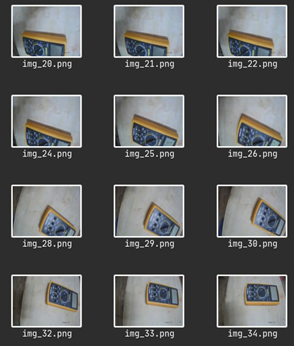
\includegraphics[width=0.3\textwidth]{input_images.png}};
    \node[above=70pt, text width=3cm,align=center] at (figure1) {Input images};

    % Second figure
    \node[draw, rectangle, blue] (figure2) at (4,2) {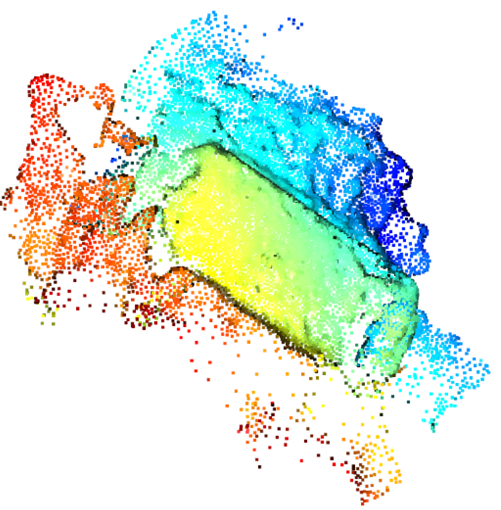
\includegraphics[width=0.25\textwidth]{dense.png}};
    \node[above=70pt, text width=100pt,align=center] at (figure2) {Dense reconstruction Output};

    % Third figure
    \node[draw, rectangle, blue] (figure3) at (8,4) {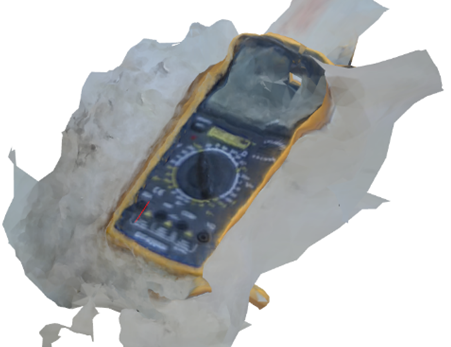
\includegraphics[width=0.27\textwidth]{output1.png}};
    \node[above=70pt,text width=100pt,align=center] at (figure3) {Texture Output from different views};

    % third figure
    \node[draw, rectangle, blue] (figure4) at (8,0) {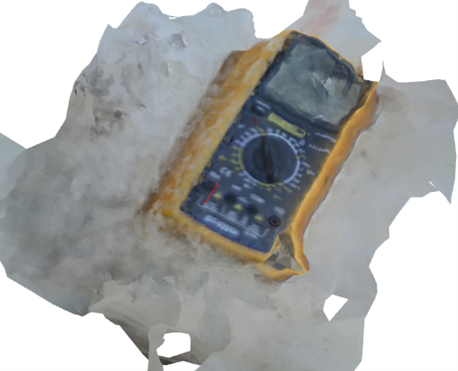
\includegraphics[width=0.27\textwidth]{output2.png}};
    
    % Arrow between figures
    \draw[->, line width=1.3pt, blue] (figure1) -- (figure2);
    \draw[->, line width=1.3pt, blue] (figure2) -- (figure3);
    \draw[->, line width=1.3pt, blue] (figure2) -- (figure4);

\end{tikzpicture}
% %
% \begin{figure}[h]
%     \centering
%     \begin{subfigure}{0.25\textwidth}
%         \centering
%         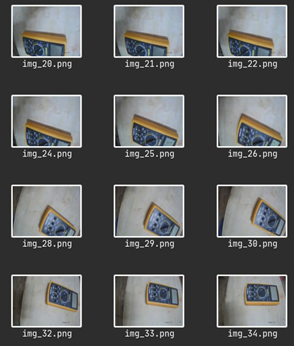
\includegraphics[width=\textwidth]{input_images.png}
%         \caption{Input images}
%     \end{subfigure}
%     \begin{tikzpicture}
%         \node[inner sep=0pt] at (0,0) {$\Rightarrow$};
%     \end{tikzpicture}
%     \hbox{\hspace{0.5cm}}
%     \begin{subfigure}{0.25\textwidth}
%         \centering
%         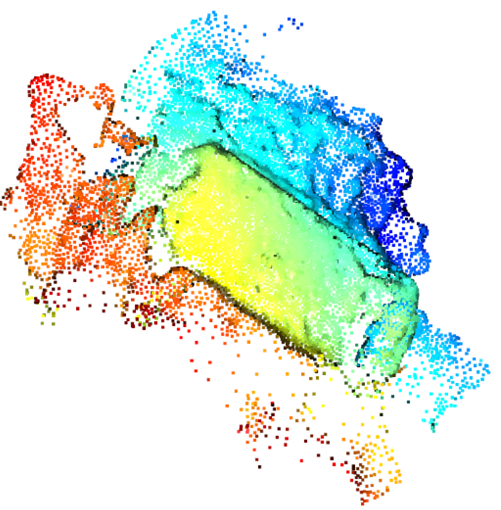
\includegraphics[width=\textwidth]{dense.png}
%         \caption{Dense reconstruction Output}
%     \end{subfigure}
%     \begin{tikzpicture}
%         \node[inner sep=0pt] at (0,500) {$\Rightarrow$};
%     \end{tikzpicture}
%     \hbox{\hspace{0.5cm}}
%     \begin{subfigure}{0.25\textwidth}
%         \centering
%         \begin{subfigure}{\textwidth}
%             \centering
%             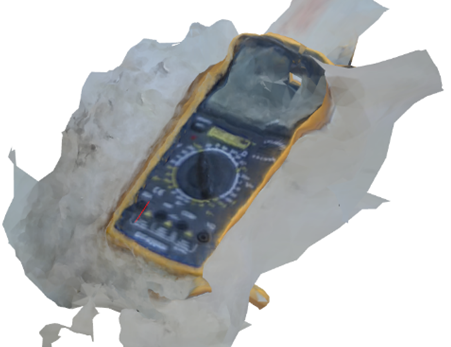
\includegraphics[width=\textwidth]{output1.png}
%         \end{subfigure}
%         \begin{subfigure}{\textwidth}
%             \centering
%             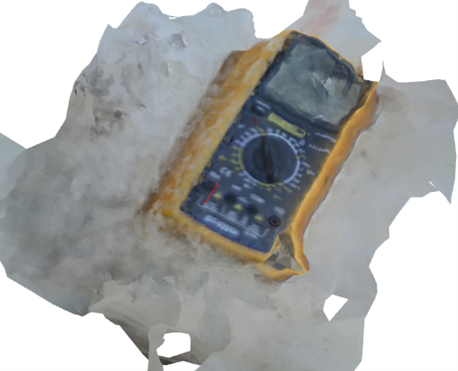
\includegraphics[width=\textwidth]{output2.png}
%         \end{subfigure}
%         \caption{Textured Output}
%     \end{subfigure}
%     \caption{Three figures with arrows and subfigures}
% \end{figure}


\end{document}